\documentclass{standalone}
\usepackage[latin1]{inputenc}
\usepackage{tikz}
\usetikzlibrary{shapes, arrows}
% Define block styles
\tikzstyle{decision} = [diamond, draw, fill=blue!20, text width=4.5em, 
    text centered, node distance=3cm, inner sep=0pt]
\tikzstyle{block} = [rectangle, draw, fill=blue!20, text width=3cm, 
    text centered, rounded corners, minimum height=4em]
\tikzstyle{info} = [rectangle, scale=0.6, text width=5cm, minimum height=4em, node distance=5.5cm]
\tikzstyle{line} = [draw, -latex']
\tikzstyle{cloud} = [draw, ellipse,fill=red!20, node distance=3cm,
    minimum height=2em]
\tikzstyle{io} = [trapezium, trapezium left angle=70, trapezium right angle=110, 
    minimum height=1cm, text centered, draw=black, fill=blue!30]

\begin{document}
    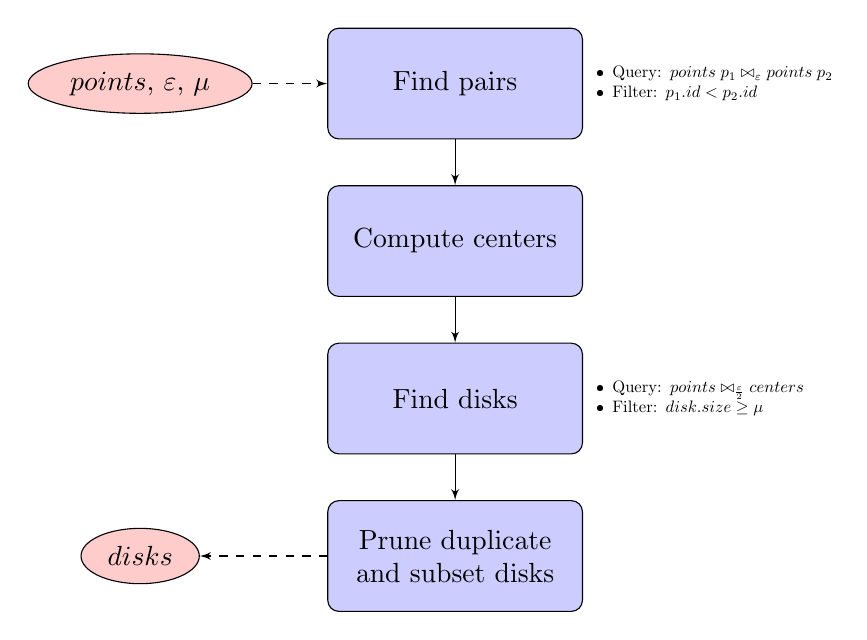
\begin{tikzpicture}[node distance = 2cm, auto]
        % Place nodes
        \node [block] (pairs) {Find pairs};
        \node [cloud, node distance=4cm, left of=pairs] (input) {$points$, $\varepsilon$, $\mu$};
        \node [block, below of=pairs] (centers) {Compute centers};
        \node [block, below of=centers] (disks) {Find disks};
        \node [block, below of=disks] (maximals) {Prune duplicate and subset disks};
        \node [cloud, node distance=4cm, left of=maximals] (output) {$disks$};
        % Info nodes
         \node [info, right of=pairs] (pairs_info) {
            \textbullet \hspace{0.1em} Query: $points\;p_1 \bowtie_{\varepsilon} points\;p_2$ \\
            \textbullet \hspace{0.1em} Filter: $p_1.id < p_2.id$ 
         };
        \node [info, right of=centers] (centers_info) { 
            %\textbullet \hspace{0.1em} See listing in appendix
        };
        \node [info, right of=disks] (disks_info) {
            \textbullet \hspace{0.1em} Query: $points \bowtie_{\frac{\varepsilon}{2}} centers$ \\
            \textbullet \hspace{0.1em} Filter: $disk.size \geq \mu $ 
         };
        \node [info, right of=maximals] (maximals_info) { 
            %\textbullet \hspace{0.1em} See listing A.2
        };
        % Draw edges
        \path [line,dashed] (input) -- (pairs);
        \path [line] (pairs) -- (centers);
        \path [line] (centers) -- (disks);
        \path [line] (disks) -- (maximals);
        \path [line,dashed] (maximals) -- (output);
    \end{tikzpicture}
\end{document}
